\section{Implementation}

\begin{figure}
  \vspace*{-3.5cm}
  \hspace*{-3cm}
  \centering
  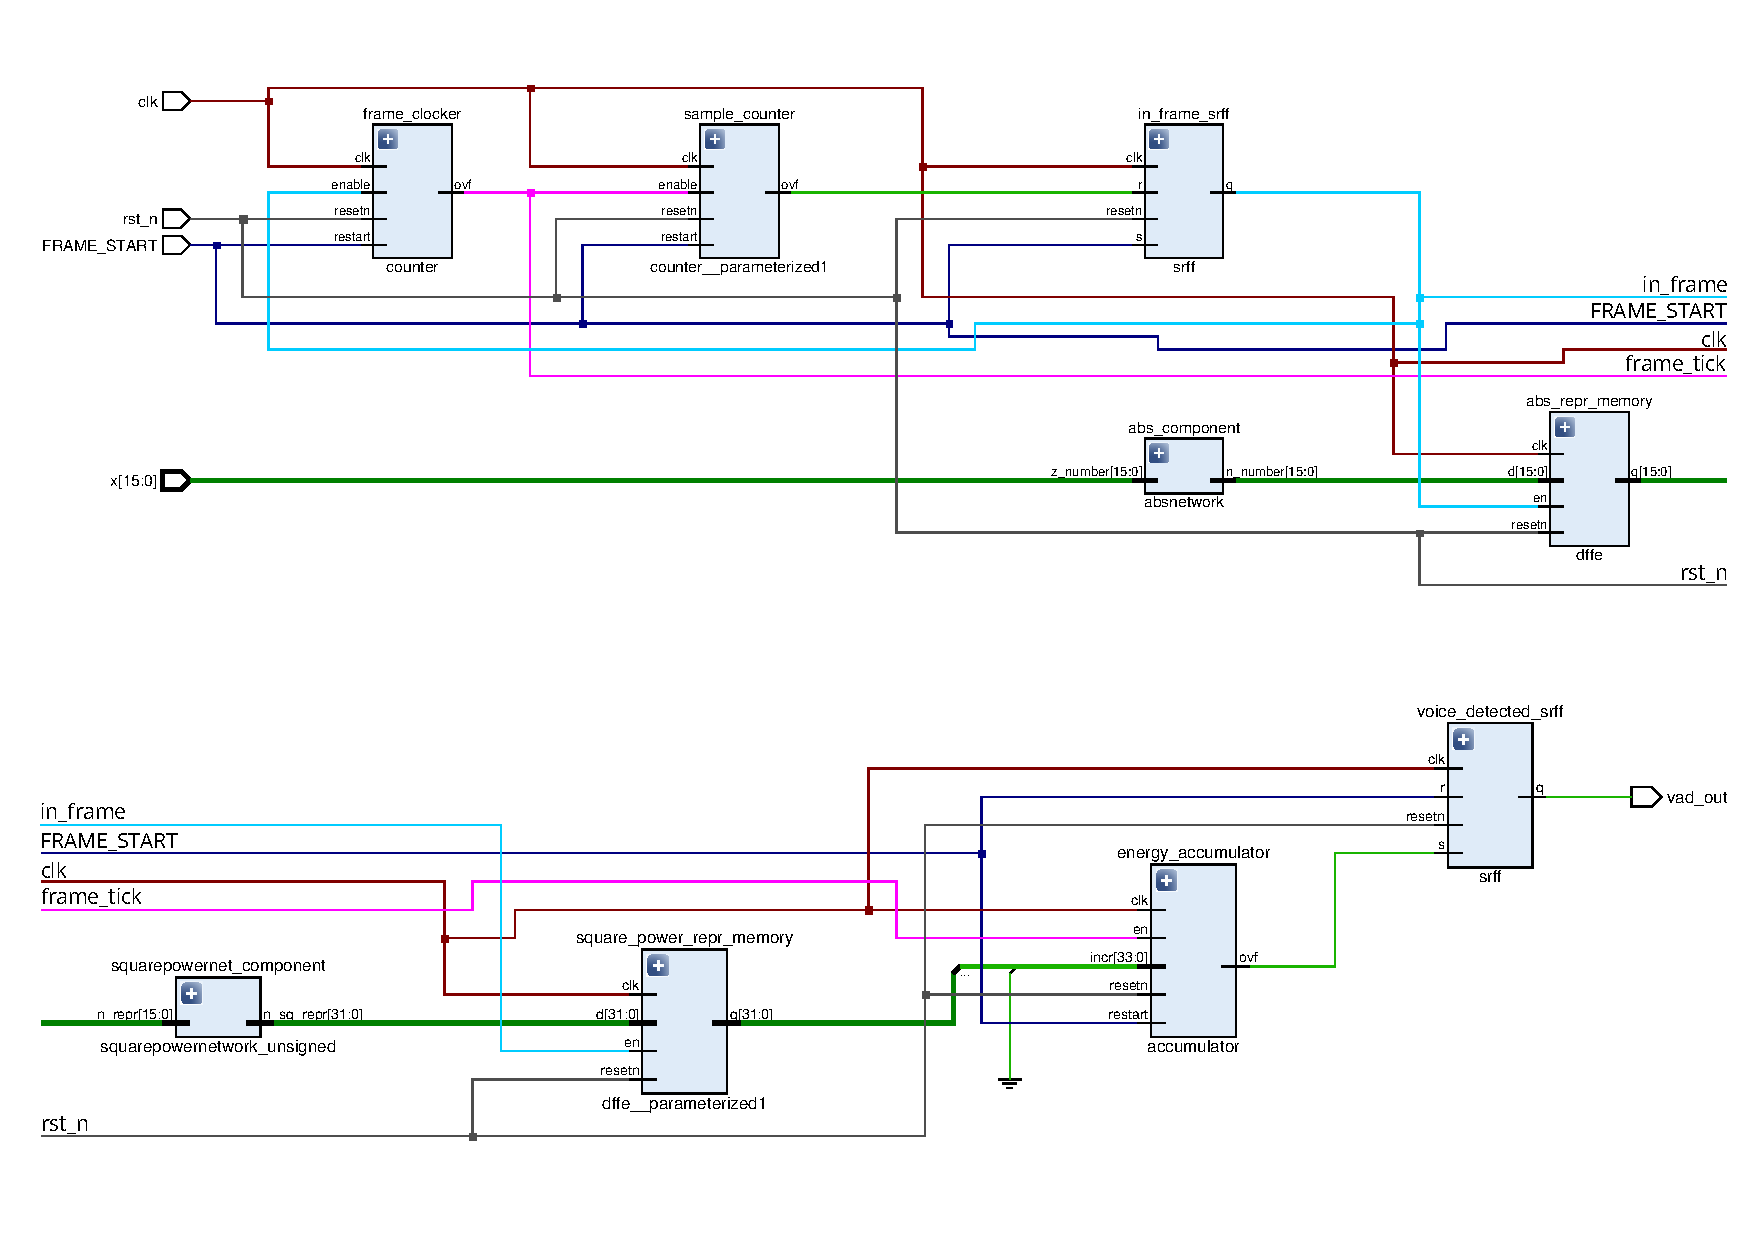
\includegraphics[width=29cm, angle=90]{figs/vad_rtl_schematic_split.pdf}
  \label{fig:schematic_rtl}
\end{figure}

This section describes the VHDL implementation using a top-down approach. The
top-view schematic of the VAD is shown in page~\pageref{fig:schematic_rtl}.

In brief, the main building blocks are:
\begin{itemize}
  \item \textbf{DFF}: D Flip-Flop.
  \item \textbf{DFFE}: D Flip-Flop with \emph{enable} input port.
  \item \textbf{DFFRE}: D Flip-Flop with \emph{enable} and \emph{r} input ports.
    The latter is a synchronous reset port like the r port in a Set-Reset Flip-Flop.
  \item \textbf{SRFF}: Set-Reset Flip-Flop.
  \item \textbf{mux\_2toN} and \textbf{mux\_4toN}: 2- and 4-ways multiplexers.
  \item \textbf{counter}: a counter that has \emph{restart} and \emph{enable}
    input ports and an \emph{overflow} output port. Default value after restart/reset
    and default value after overflow can be configured as parameters.
  \item \textbf{accumulator}: an accumulator that has \emph{data}, \emph{restart} and \emph{enable}
    input ports and an \emph{overflow} output port. Default value after restart/reset
    can be configured as a parameter.
  \item \textbf{squarepowernetwork\_unsigned}: performs the square of an unsigned
    number.
  \item \textbf{absnetwork}: performs the absolute value.
  \item \textbf{absnetwork\_approx}: performs the absolute value using the approximation
    of \cref{sec:opt-abs}.
  \item \textbf{rtl\_adder}: performs the sum of two unsigned numbers.
\end{itemize}

\subsection{VAD}
The VAD is made of the following components:
\begin{itemize}
  \item \textbf{in\_frame\_srff}: this \emph{SRFF} is set by \texttt{FRAME\_START} when
    the frame is started and is reset when the frame ends (see \emph{sample\_counter}).
    This component's output serves as the enabler of the \emph{frame\_counter}
    and all pipeline registers.
  \item \textbf{frame\_clocker}: this \emph{counter} is the frequency divider
    that ticks at the middle of every frame. It's output enables the
    \emph{sample\_counter} and the \emph{energy\_accumulator}.
  \item \textbf{sample\_counter}: this \emph{counter} counts the number of samples
    and, when the frame ends, it sends a signal to reset the \emph{in\_frame\_srff}.
  \item \textbf{energy\_accumulator}: this \emph{accumulator} sums up the
    squares of the input samples and overflows once the energy threshold is
    trespassed. It is reset at the beginning of every frame.
  \item \textbf{voice\_detected\_srff}: this \emph{SRFF} is set when the
    \emph{energy\_accumulator} overflows, signaling the trespassing of the
    energy threshold and, hence, the detection of voice in the signal. It is
    reset with \texttt{FRAME\_START}. It is directly connected to the output.
  \item \textbf{abs\_component}: performs the absolute value.
  \item \textbf{squarepowernet\_component}: performs the squaring.
  \item \textbf{abs\_repr\_memory} and \textbf{square\_power\_repr\_memory}:
    they are pipeline registers. They are not necessary but their presence
    improves the performance of the design. Refer to \cref{sec:pipeline} for
    more information.
\end{itemize}

\subsection{Counter}
\begin{figure}[]
  \centering
  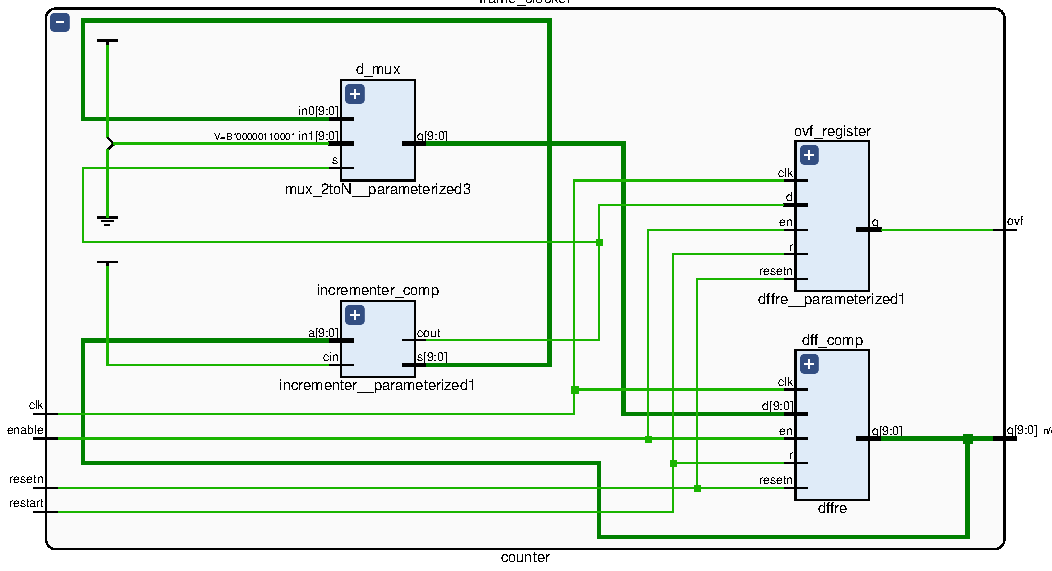
\includegraphics[width=\textwidth]{figs/counter_schematic.pdf}
  \caption{RTL schematic for the counter component.}
  \label{fig:counter}
\end{figure}

\cref{fig:counter} shows the internal implementation of the counter, where you
can see the following components:
\begin{itemize}
  \item \textbf{dff\_comp}: a \emph{DFFRE} that holds the current state of the
    counter. It is enabled if and only if the counter is enabled.
  \item \textbf{ovf\_register}: a \emph{DFFRE} that buffers the overflow of the
    \emph{incrementer\_comp}. It is enabled if and only if the counter is enabled.
  \item \textbf{incrementer\_comp}: an \emph{incrementer} that increments the
    output of the \emph{dff\_comp}.
  \item \textbf{d\_mux}: a \emph{2-way multiplexer} that is used to restart the
    counter from a predefined value when the incrementer overflows. If there is
    no overflow, its output is the output of the incrementer, otherwise it is
    the predefined default value.
\end{itemize}

Furthermore, it is important to note that both the default value after reset
or restart and the default value after overflow can be set as parameters.
This enables the counter to have basically any predefined period.

\subsection{Accumulator}
\begin{figure}[]
  \centering
  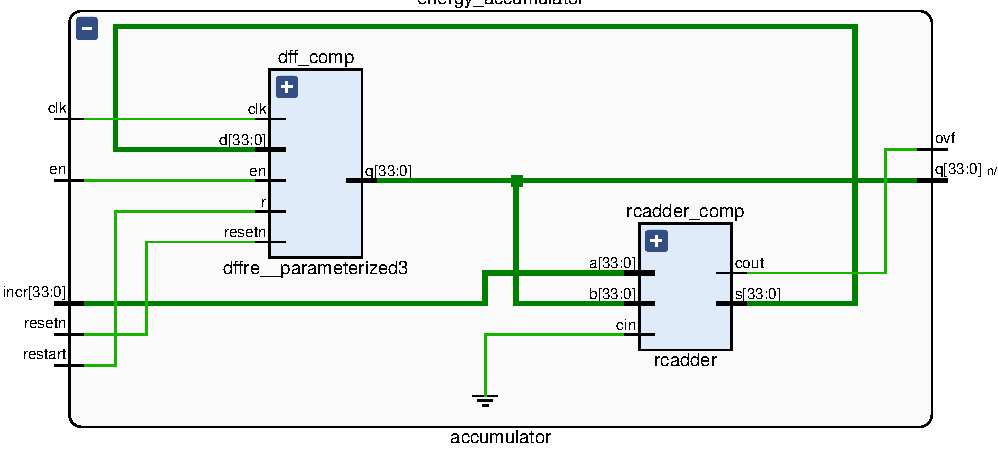
\includegraphics[width=\textwidth]{figs/accumulator_schematic.pdf}
  \caption{RTL schematic for the accumulator component.}
  \label{fig:accumulator}
\end{figure}

\cref{fig:accumulator} shows the internal implementation of the accumulator, where you
can see the following components:
\begin{itemize}
  \item \textbf{dff\_comp}: a \emph{DFFRE} that holds the current state of the
    accumulator. It is enabled if and only if the accumulator is enabled.
  \item \textbf{ovf\_register}: a \emph{DFFRE} that buffers the overflow of the
    \emph{rcadder\_comp}. It is enabled if and only if the accumulator is enabled.
  \item \textbf{rcadder\_comp}: a \emph{ripple-carry adder} that adds the input
    \emph{incr} to the content of \emph{dff\_comp}. The overflow output is
    directly connected with the output port.
\end{itemize}

Furthermore, it is important to note that the default value after reset
or restart can be set as a parameter.
This enables the accumulator to overflow as soon as the threshold is trespassed.

\subsection{DFFRE and DFFE}
\begin{figure}[]
  \centering
  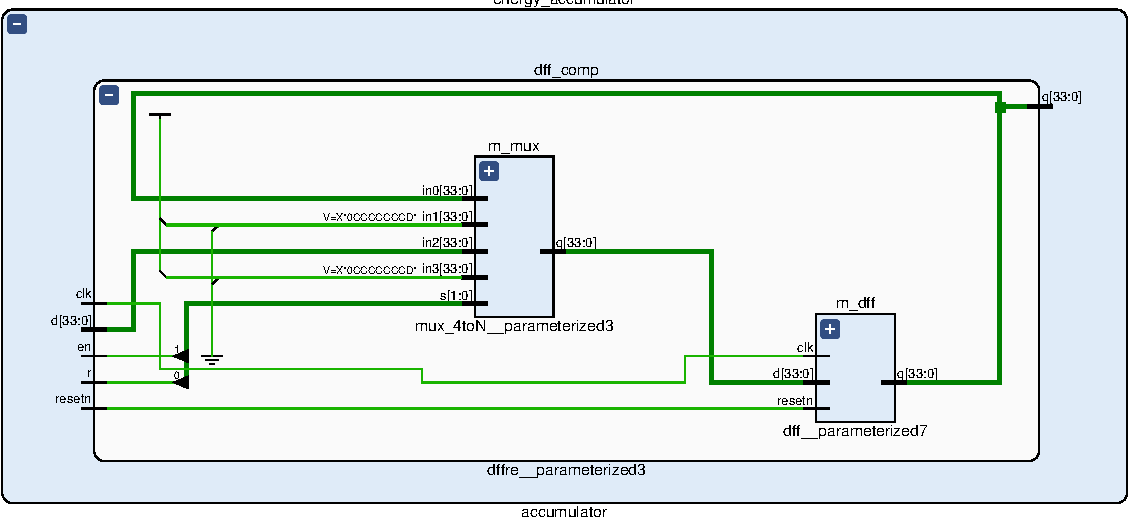
\includegraphics[width=\textwidth]{figs/dffre_schematic.pdf}
  \caption{RTL schematic for the DFFRE component.}
  \label{fig:dffre}
\end{figure}

The ``DFFE'' is a D Flip-Flop with an \emph{enable} input port,
in addition to the classic \emph{data}, \emph{clk} and \emph{rst\_n}.
The \emph{enable} port controls the sensitivity of the DFF on the input: if
\emph{enable} is 0, the DFF will keep its value.

The ``DFFRE'' has in addition a \emph{r} input port. The \emph{r} port is, instead,
a synchronous reset port like the \emph{r} port in a \emph{Set-Reset Flip-Flop}.

Both the \emph{DFFE} and the \emph{DFFRE} are implemented using a multiplexer that
chooses the input to the DFF depending on the value of the \emph{enable} and
\emph{r} inputs, as it can be seen in \cref{fig:dffre}.

When the flip-flop is reset, by either using \emph{rst\_n} or \emph{r}, its
content will be reset to a predefined value, that can be set as a parameter.

\subsection{Pipeline registers}
\label{sec:pipeline}

The registers \textbf{abs\_repr\_memory} and \textbf{square\_power\_repr\_memory}
were added as pipeline registers to split the long combinatorial chain. This 
reduces the critical path and the power consumption of the component since 
oscillations in the input are not propagated through the entire chain.